\documentclass{standalone}
\usepackage{tikz}
\begin{document}
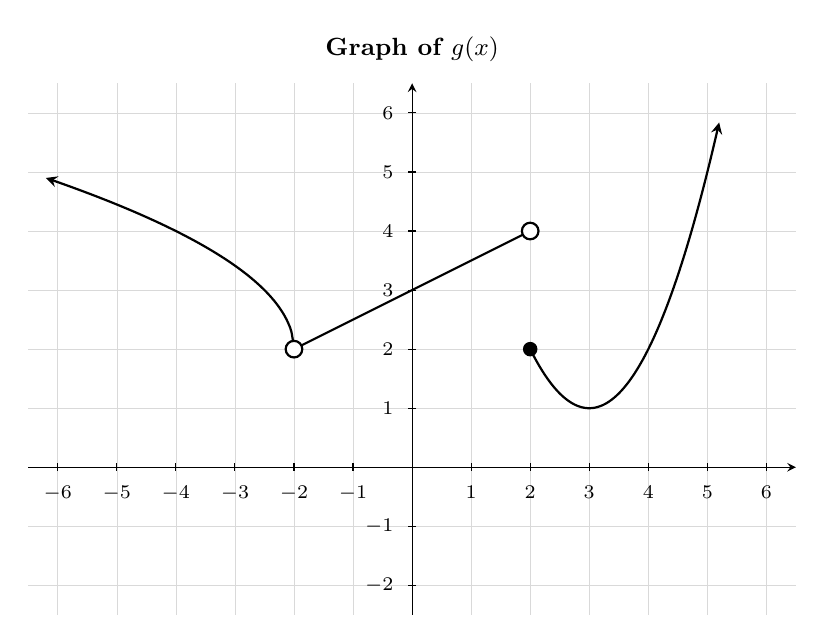
\begin{tikzpicture}[>=stealth, scale=0.75]

% Grid
\draw[gray!30, very thin, step=1] (-6.5,-2.5) grid (6.5,6.5);

% Axes
\draw[->] (-6.5,0) -- (6.5,0);
\draw[->] (0,-2.5) -- (0,6.5);

% X-axis tick labels
\foreach \x in {-6,-5,-4,-3,-2,-1,1,2,3,4,5,6} {
  \draw (\x,0.07) -- (\x,-0.07);
  \node[below, font=\scriptsize] at (\x,-0.15) {$\x$};
}

% Y-axis tick labels
\foreach \y in {-2,-1,1,2,3,4,5,6} {
  \draw (0.07,\y) -- (-0.07,\y);
  \node[left, font=\scriptsize] at (-0.15,\y) {$\y$};
}

% Title
\node[font=\small\bfseries, above] at (0,6.7) {Graph of $g(x)$};

\begin{scope}
\clip (-6.5,-2.5) rectangle (6.5,6.5);

% Left piece: square root, vertex (-2,2), through (-4,4): y = sqrt(2)*sqrt(-(x+2)) + 2 for x < -2
% arrow at the left (upper) end
\draw[<-, thick, smooth, samples=100, domain=-6.2:-2, variable=\x]
  plot ({\x},{sqrt(2)*sqrt(-(\x+2))+2});

% Middle piece: line, y = x/2 + 3, slope 1/2, from (-2,2) to (2,4)
\draw[thick] (-2,2) -- (2,4);

% Right piece: quadratic, y = (x-3)^2 + 1 for x >= 2
% vertex at (3,1); starts at (2,2); arrow at upper-right
\draw[->, thick, smooth, samples=100, domain=2:5.2, variable=\x]
  plot ({\x},{(\x-3)*(\x-3)+1});

\end{scope}

% Open circle at (-2,2): sqrt and line both exclude x=-2
\draw[fill=white, draw=black, thick] (-2,2) circle (4pt);

% Open circle at (2,4): right end of line (excluded)
\draw[fill=white, draw=black, thick] (2,4) circle (4pt);

% Filled dot at (2,2): start of quadratic (included)
\fill[black] (2,2) circle (3.5pt);

\end{tikzpicture}
\end{document}
